\chapter{QHD-I}

This chapter will describe the derivation of an equation of state from the QHD-I parameter set, as described within \autocite{diener_2008}.

\section{Introduction}


\section{Derivation of equations of motion}

The Euler-Lagrange equations, for a Lagrange density $\Lag$ over a classical field $\varphi_\alpha$, are given by
\begin{align}\label{eqn: ELE}
    \p_\nu\qty(\pdv{\Lag}{(\p_\nu \varphi_\alpha)}) - \pdv{\Lag}{\varphi_\alpha} = 0.
\end{align}
From \autocite[p. 56]{diener_2008}, we have the Lagrangian density of QHD-I
\begin{align} \label{eqn: QH, LD,QHD1}
    \Lag & = \bar{\psi} \bqty{\gamma_\mu(i\p^\mu -g_\nu V^\mu) - (M-g_s\phi)} \psi \nonumber\\
    & \quad + \frac{1}{2} \pqty{\p_\mu \phi \p^\mu \phi - m_s^2 \phi^2} - \frac{1}{4} V_{\mu\nu}V^{\mu\nu} + \frac{1}{2} m_\omega^2 V_\mu V^\mu,
\end{align}
where $V_{\mu\nu}\Def\p_\mu V_\nu (x) - \p^\nu V_\mu(x)$. To determine the equations of motion for this system, we must apply \eqref{eqn: ELE} to \eqref{eqn: QH, LD,QHD1} for each unique field in the system
\begin{align*}
    \varphi_\alpha = \begin{cases}
        \phi(x) &: \quad \text{scalar meson field,}\\
        V^\mu(x) &: \quad \text{vector meson field,}\\
        \psi(x) &: \quad \text{baryon field,}\\
        \bar\psi(x) &: \quad \text{Dirac adjoint baryon field,}\\
    \end{cases}
\end{align*}
where $\bar\psi(x) \Def \psi^\dagger(x)\gamma^0$, the \emph{Dirac adjoint.}

For the scalar meson field, when $\varphi_\alpha = \phi(x)$, the first term in \eqref{eqn: ELE} gives
\begin{align*}
    \p_\nu \pqty{\pdv{\Lag}{(\p_\nu \phi)}} = \frac{1}{2} \bqty{\pdv{(\p_\nu \phi)}\pqty{\p_\mu \p^\mu \phi}} = \p_\nu \p^\nu \phi,
\end{align*}
while the second term gives
\begin{align*}
    \pdv{\Lag}{\phi} = \bar\psi[+g_s]\psi + \frac{1}{2}\pqty{-m_s(2\phi)} = g_s \bar\psi \psi - m_s\phi.
\end{align*}
Combining, we get the first equation of motion,
\begin{align}\label{eqn: eom,sm}
    \p_\nu \pqty{\pdv{\Lag}{(\p_\nu \phi)}} - \pdv{\Lag}{\phi} = \p_\nu \p^\nu \phi - (g_s\bar\psi \psi - m_s\phi) = 0 \goesto \p_\nu \p^\nu \phi + m_s \phi = g_s \bar\psi \psi.
\end{align}
This is the form given in \autocite{diener_2008} (8.1a).

For the vector meson field, when $\varphi_\alpha = V_\mu$, the first term in \eqref{eqn: ELE} gives
\begin{align*}
    \p_\nu \pqty{\pdv{\Lag}{(\p_\nu V_\mu)}} = \p_\nu V^{\mu\nu},
\end{align*}
after many simplifications, including using the definition of $V^{\mu\nu}$ and the relabelling of indices. The second term gives
\begin{align*}
    \pdv{\Lag}{V_\mu} = \pdv{}{V_\mu}\bar\psi\bqty{\gamma_\alpha(-g_v V^\alpha) + \frac{1}{2} m_\omega^2 V^\alpha V_\alpha} = -g_v \bar\psi \gamma^\mu \psi + m_\omega^2 V^\mu,
\end{align*}
and combining we have
\begin{align}\label{eqn: vEOM, intermediate}
    \p_\nu \pqty{\pdv{\Lag}{(\p_\nu V_\mu)}} - \pdv{\Lag}{V_\mu} = \p_\nu V^{\mu\nu} - (-g_v \bar\psi \gamma^\mu \psi + m_\omega^2 V^\mu) = 0.
\end{align}
However, this is not the form given in \autocite{diener_2008}; to reach his form, we leverage the anti-symmetry of $V_{\mu\nu}$, namely
\begin{align*}
    V_{\mu\nu} = - V_{\nu\mu}.
\end{align*}
Therefore, we make the above substitution, multiply \eqref{eqn: vEOM, intermediate} by $-1$, and send $\mu \leftrightarrow \nu$ to obtain
\begin{align}\label{eqn: eom,vm}
    \p_\mu V^{\mu\nu} + m_\omega^2 V^\nu = g_v \bar\psi \gamma^\nu \psi,
\end{align}
as given in \cite{diener_2008} (8.1b).

Next, we have the two equations of motion from the baryon field. For $\varphi_\alpha = \bar\psi$, applying \eqref{eqn: ELE} is straight forward, as there is no $\p_\nu \bar\psi$ dependence in $\Lag$, so the first term in \eqref{eqn: ELE} is zero. Thus, we obtain
\begin{align}\label{eqn: eom,barpsi}
    \p_\nu \pqty{\pdv{\Lag}{(\p_\nu \bar\psi)}}  - \pdv{\Lag}{\bar\psi} = \bqty{\gamma_\mu(i\p^\mu - g_v V^\mu) - (M-g_s\phi)} \psi = 0.
\end{align}
For the final case, when $\varphi_\alpha = \psi$, the first term in \eqref{eqn: ELE} gives
\begin{align*}
    \p_\nu \pqty{\pdv{\Lag}{(\p_\nu \psi)}} = \p_\nu\bqty{\pdv{}{(\p_\nu\psi)}\bar\psi i \gamma_\alpha \p^\alpha \psi} = i\p_\nu \bar\psi \gamma^\nu,
\end{align*}
while the second gives
\begin{align*}
    \pdv{\Lag}{\psi} = \bar\psi\bqty{\gamma_\mu(i\p^\mu - g_v V^\mu) - (M-g_s\phi)}.
\end{align*}
Combining, we get our fourth equation
\begin{align}\label{eqn: eom,psi}
    i \p_\nu \bar\psi \gamma^\nu -\bar\psi\bqty{\gamma_\mu(i\p^\mu - g_v V^\mu) - (M-g_s\phi)} = 0.
\end{align}
In summary, here are the four equations of motion for QHD-I:
\begin{align*}
    &\p_\nu \p^\nu \phi + m_s^2\phi = g_s\bar{\psi}\psi,\tag{\ref{eqn: eom,sm}}\\
    &\p_\mu V^{\mu\nu} + m_\omega^2 V^\nu = g_v \bar\psi \gamma^\nu \psi,\tag{\ref{eqn: eom,vm}}\\
    &\bqty{\gamma_\mu(i\p^\mu -g_v V^\mu) - (M-g_s\phi)} \psi = 0,\tag{\ref{eqn: eom,barpsi}}\\
    & i \p_\nu \bar\psi \gamma^\nu -\bar\psi\bqty{\gamma_\mu(i\p^\mu - g_v V^\mu) - (M-g_s\phi)} = 0. \tag{\ref{eqn: eom,psi}}
\end{align*}
The first three are given in \autocite{diener_2008}.

\section{Relativistic Mean Field Simplifications}

In \autocite{diener_2008} \S 8.3, we find that the equations of motion listed above are very difficult to solve in their current form. To make them more manageable, we approximate them with ``relativistic mean field'' (RMF) simplifications, where we take each field to be its ground state expectation value. For the meson fields, this simplification yields
\begin{align}
    \phi &\goesto \bra{\Phi} \phi \ket{\Phi} = \expval{\phi} \Def \phi_0, \\
    V_\mu & \goesto \bra{\Phi} V_\mu \ket{\Phi} = \expval{V_\mu} \Def \delta_{\mu 0} V_0,
\end{align}
where $\ket{\Phi}$ represents the ground state. These results arise from arguing that, in their ground states, $\phi$ and $V_\mu$ should be independent of space and time, as the system is bot uniform and stationary; therefore, $\phi_0$ and $V_0$ are constants. Furthermore, because the system is at rest and the baryon flux, $\bar\psi\gamma^i\psi$, is zero, the spatial components of the expected value of $V_\mu$, $\expval{V_\mu}$, must vanish \autocite{diener_2008}.

For the baryon field, a ``normal order'', i.e. normalized, expectation value must be taken, as because otherwise, the vacuum would be taken into account and the traditional expectation value would diverge. This ``normal ordered'' expectation value is denoted with a ``:''. Thus, these are the expectation values for the baryon field
\begin{align}
    \bar\psi\psi &\goesto \bra{\Phi}\!:\!\psi\psi\!:\!\ket{\Phi} = \expval{\bar\psi\psi}.\\
    \bar\psi\gamma^\mu \psi &\goesto \bra{\Phi}\!:\!\psi\gamma^\mu\psi\!:\!\ket{\Phi} = \expval{\psi\gamma^0\psi}.
\end{align}

Given these simplifications, we can rewrite the equations of motion given in equations \eqref{eqn: eom,sm}, \eqref{eqn: eom,vm}, \eqref{eqn: eom,barpsi}, and \eqref{eqn: eom,psi} as

\begin{align}
    & m_s^2 \phi_0^2 = g_s\expval{\bar\phi\phi}\\
    & m_\omega^2 V_0 = g_v\expval{\bar\phi\gamma^0\phi}\\
    & \bqty{i\gamma_\mu\p^\mu - g_v\gamma_0 V_0 - (M - g_s\phi_0)}\psi = 0\\
    & i \p_\mu \bar\psi \gamma^\mu -\bar\psi\bqty{i\gamma_\mu\p^\mu - g_v \gamma_0V_0 - (M-g_s\phi)} = 0.
\end{align}

From \autocite[p. 40]{diener_2008} (6.14), where we consider the star to be a spherically symmetric fluid with velocity $\vb{v}=0$, we get the following forms for $\epsilon$ and $P$
\begin{align}\label{eqn: eps and P defs}
    \epsilon = \expval{T^{00}}, \quad P = \frac{1}{3}\expval{T^{ii}},
\end{align}
where $T^{\mu\nu}$ is the energy-momentum tensor, given by \autocite[p. 40]{diener_2008} (6.13), is
\begin{align}\label{eqn: emt}
    T^{\mu\nu} = \pdv{\Lag}{(\p_\mu \varphi_\alpha)}\p^\nu \varphi_\alpha - \Lag \eta^{\mu\nu}.
\end{align}

Given the simplifications at the beginning of this section, we can form the Lagrangian Density for an RMF QHD-1 framework, a modification of \eqref{eqn: QH, LD,QHD1}. Making the substitutions $\phi\to \phi_0$ and $V_\mu = \delta_{\mu 0 } V_0$, we get
\begin{align}
    \Lag_\text{RMF} = \bar\psi \bqty{i\gamma_\mu\p^\mu - g_v \gamma_0 V_0 - (M-g_s\phi_0)} \psi - \frac{1}{2} m_s^2 \phi_0^2 + \frac{1}{2} m_\omega^2 V_0^2,
\end{align}
as given in Diener. Next, we form the energy momentum tensor using \eqref{eqn: emt}. We use $\varphi_\alpha \in \{ \phi_0, V_0, \psi\}$. There is no dependence of $\Lag_\text{RMF}$ on the derivatives of $\phi_0$ and $V_0$, so for those values of $\varphi_\alpha$, the first term in \eqref{eqn: emt} is zero. For $\psi$, however, there is a $\p^\mu$ within the first term in the brackets, so we must deal with a $\p_\mu \psi$ derivative. 

To start, we distribute the $\psi$ and $\bar\psi$ into the brackets, and notice that only the first term has any $\p_\mu \psi$ dependence, so
\begin{align}
    \pdv{\Lag_\text{RMF}}{(\p_\mu \psi)} \p^\nu \varphi_\alpha & = \pdv{(\p_\mu \psi)}\bqty{\bar\psi i \gamma_\sigma \p^\sigma\psi}\p^\nu \psi + \cancelto{0}{\pdv{(\p_\mu \psi)}\bqty{\cdots}} \p^\nu \psi = i\bar\psi\gamma^\mu \p^\nu \psi.
\end{align}
The second term in \eqref{eqn: emt} is straightforward. However, we can simplify by substituting \ref{eqn: eom,barpsi} into the Lagrangian density when we form this term, such that
\begin{align}
    \Lag \eta^{\mu\nu} &= \eta^{\mu\nu}\pqty{\bar\psi \bqty{i\gamma_\mu\p^\mu - g_v \gamma_0 V_0 - (M-g_s\phi_0)} \psi - \frac{1}{2} m_s^2 \phi_0^2 + \frac{1}{2} m_\omega^2 V_0^2}\nonumber\\
    & = \eta^{\mu\nu} \pqty{- \frac{1}{2} m_s^2 \phi_0^2 + \frac{1}{2} m_\omega^2 V_0^2}.
\end{align}
Therefore, by \eqref{eqn: emt}, the \textsc{rmf} energy momentum tensor takes the form
\begin{align}
    T^{\mu\nu}_\text{RMF} & =i\bar\psi\gamma^\mu \p^\nu \psi - \eta^{\mu\nu} \pqty{- \frac{1}{2} m_s^2 \phi_0^2 + \frac{1}{2} m_\omega^2 V_0^2}.
\end{align}
If we now use this result in \eqref{eqn: eps and P defs}, we obtain equations for $\epsilon$ and $P$
\begin{align}
    \epsilon & = \expval{T^{00}} = \expval{i\bar\psi\gamma^0 \p^0 \psi} + \frac{1}{2} m_s^2 \phi_0^2 - \frac{1}{2} m_\omega^2 V_0^2,\\
    P &= \frac{1}{3}\expval{T^{ii}} = \expval{i\bar\psi\gamma^i \p^i \psi}  - \frac{1}{2} m_s^2 \phi_0^2 + \frac{1}{2} m_\omega^2 V_0^2.
\end{align}
Now that we have expressions for $\epsilon$ and $P$, we need to evaluate the expectation values in order to calculate numerical values for the equation of state.


\medskip
\JN{MORE HERE. EXPLAIN EVALUATION OF EXPECTATION VALUES.}
% simplifications for baryon field
% derivation of energy momentum tensor and lagrangian for RMF
% derivation of energy density and pressure from EMT
% calculation of expectation values
\medskip

After evaluating these expectation values, we have
\begin{align}
    \phi_0 &= \frac{g_s}{m_s^2} \frac{\gamma}{2\pi^2}\int_0^{k_f} \dd{k} \frac{k^2 m^*}{\sqrt{k^2 + m^{*2}}}, \label{eqn: rmf,phi0} \\
    V_0 &= \frac{g_v}{m_\omega^2} \rho, \label{eqn: rmf,V0}
\end{align}
where once again, $m^* \Def M - g_s \phi$, the \emph{reduced mass}, and $\rho$ is the nucleon number density. If we assume spherical symmetry, a reasonable condition for the study of star-like systems, we get thee following expressions
\begin{align}
    \epsilon & = \frac{1}{2} m_s^2 \phi_0^2 + \frac{1}{2} m_\omega^2 V_0^2 + \frac{\gamma}{2\pi^2} \int_0^{k_f} \dd{k} k^2 \sqrt{k^2 + m^{*2}}, \label{eqn: rmf,eps}\\
    P & = -\frac{1}{2} m_s^2 \phi_0^2 + \frac{1}{2} m_\omega^2 V_0^2 + \frac{1}{3} \pqty{\frac{\gamma}{2\pi^2} \int_0^{k_f} \dd{k}\frac{k^4}{\sqrt{k^2 + m^{*2}}}}. \label{eqn: rmf,p}
\end{align}
In the next section, we will use these expressions to generate values for this equation of state.

\section{Numerical generation of the equation of state}

Throughout this section, we will extensively reference \autoref{ch: qhd1 code}. Any line numbers directly reference the code presented there.

% We now wish to generate tabulated values of the equation of state using the equations for $\epsilon, P$ and $\phi_0$ at the end of the previous section. To do so, we first wish to find analytical forms for the integrals present in each of those equations, respectively. The aforementioned integrals are the following
% \begin{align}
%     \int_{0}^{k_f} \dd{k} \frac{k^2 m^*}{\sqrt{k^2 + m^{*2}}}, \quad\int_{0}^{k_f} \dd{k} \frac{k^4}{\sqrt{k^2 + m^{*2}}},
%     \quad\int_{0}^{k_f} \dd{k} k^2\sqrt{k^2 + m^{*2}}.
% \end{align}
% We integrate each of these using Mathematica, giving it the assumptions that $k_f > 0$ and that $\Re[m^*] > 0$. This gives these explicit, closed forms
% \begin{align}
%     \int_{0}^{k_f} \dd{k} \frac{k^2 m^*}{\sqrt{k^2 + m^{*2}}} &= \frac{1}{2} m^* \pqty{k_f \sqrt{k_f^2 + m^{*2}} - m^{*2}\ln\bqty{\frac{k_f + \sqrt{k_f+m^{*2}}}{k_f}}} \\
%     \int_{0}^{k_f} \dd{k} \frac{k^4}{\sqrt{k^2 + m^{*2}}} &= \frac{1}{8} \pqty{k_f(2k_f^2 - 3m^{*2}) - 3m^{*4}\ln\bqty{\frac{k_f + \sqrt{k_f+m^{*2}}}{k_f}}}\\
%     \quad\int_{0}^{k_f} \dd{k} k^2\sqrt{k^2 + m^{*2}} &= \frac{1}{8} \pqty{k_f \sqrt{k_f^2 + m^{*2}}\qty(2k_f^2 + m^{*2}) - m^{*4}\ln\bqty{\frac{k_f + \sqrt{k_f+m^{*2}}}{k_f}}}
% \end{align}

We now wish to generate tabulated values of the equation of state using the equations for $\epsilon, P$ and $\phi_0$ at the end of the previous section. Simply, this process requires looping through various values of $k_f$; at each iteration, we find the corresponding value of $\phi_0$ by using a root finding routine on \eqref{eqn: rmf,phi0}, as $m^*$ depends on $\phi_0$, then computing $V_0$ independently using \eqref{eqn: rmf,V0}, and then finally substituting those values into \eqref{eqn: rmf,eps} and \eqref{eqn: rmf,p} and storing those values. After creating a table of values for $\epsilon$ and $P$, we can verify the validity of the equation of state by solving the TOV equations and comparing the results of static solutions, mass-radius curves, and mass-pressure curves to other, previously calculated equations of state. An in-depth description of the TOV equations and their implementation is given in \autoref{ch: static solutions}.

To begin, we choose a value of $k_f$ for the entirety of the iteration; for sake of example, we take $k_f = 1$. Then, we find the value of $\phi_0$ for that $k_f$ value. We define a function in Python for $\phi_0$ from \eqref{eqn: rmf,phi0}. This is given between lines 20 and 28.

While most of the function is straight forward, lines 23-26 may be cryptic without context. These lines are responsible for numerically computing the integral at the end of \eqref{eqn: rmf,phi0}, given the current $k_f$ value. \code{f(x)} is simply a function definition for the integrand of that integral, while line 26 uses the SciPy function \code{quad} to numerically integrate \code{f} from $0$ to $k_f$. \code{quad} returns a tuple containing both the numerical value of the integration and the bounds on that value's error, so we unpack it to get the value we want and call it \code{integral}. 

To determine the value of $\phi_0$, we must use a root finding routine because in \eqref{eqn: rmf,phi0}, $\phi_0$ appears on both sides of the equation. Thus, we subtract all terms to one side of the equality such that is set equal to zero. This function will later be passed to SciPy function called \code{root} that will find when this function equals zero, meaning we have the desired value of $\phi_0$.

For the remaining parameters, $V_0$, $P$, and $\epsilon$, we simply define functions to determine their values. In the equations for $P$ and $\epsilon$, we again use numerical integration using $\quad$ to determine the value of each integral, just as with the $\phi_0$ equation.

Now we are ready to calculate values for $P$ and $\epsilon$. We create an array of $k_f$ values, and loop through each. During every iteration, we calculate the root of the $\phi_0$ function, which gives us $\phi_0$, and we use that value, as well as the value of $V_0$ to determine the values of $P$ and $\epsilon$.  These values are saved and written to file. Notably, our root finding needs an initial guess, so we use the previously determined value of $\phi_0$ as the guess for the current iteration, as we know it will be relatively close.

After tabulating values for this QHD-1 equation of state, we can create mass-radius and mass-pressure curves, as derived in \autoref{ch: static solutions}. This produces the results given in \autoref{fig: qhd1 mass radius pressure}.

\begin{figure}[h!]
    \centering
    \begin{subfigure}{.5\textwidth}
        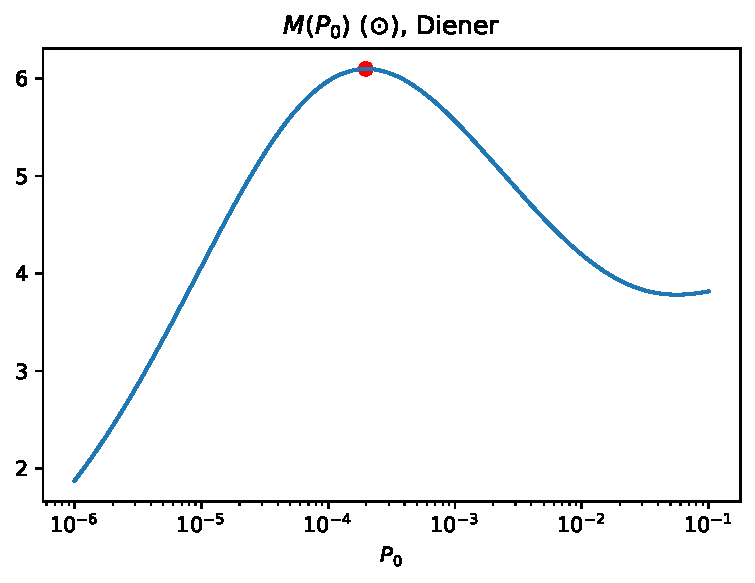
\includegraphics[width=\textwidth]{images/qhd1/p0_analysis.pdf}
    \end{subfigure}%
    \begin{subfigure}{.5\textwidth}
        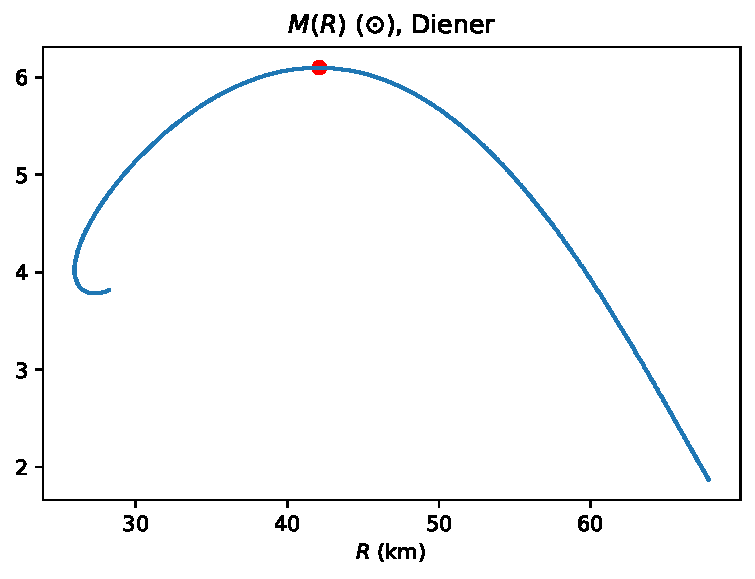
\includegraphics[width=\textwidth]{images/qhd1/r_analysis.pdf}
    \end{subfigure}
    \caption{The mass-pressure curve (left) and mass-radius curve (right) for the QHD-1 equation of state given in \autocite{diener_2008}.}
    \label{fig: qhd1 mass radius pressure}
\end{figure}

From these plots and this analysis, we calculate the critical (maximum) mass that this EOS predicts to be \SI{6.1}{\odot} with a critical radius of \SI{42.1}{km}.

\section{Analysis}

